\documentclass[12pt]{article}
\usepackage{amssymb,amsfonts,amsmath, psfrag,eepic,colordvi,graphicx,epsfig,ytableau}
\usepackage{amssymb,latexsym,graphics,array}
\usepackage{tikz,ifthen}
\usepackage{pgfplots}
\usetikzlibrary{math}

\begin{document}

		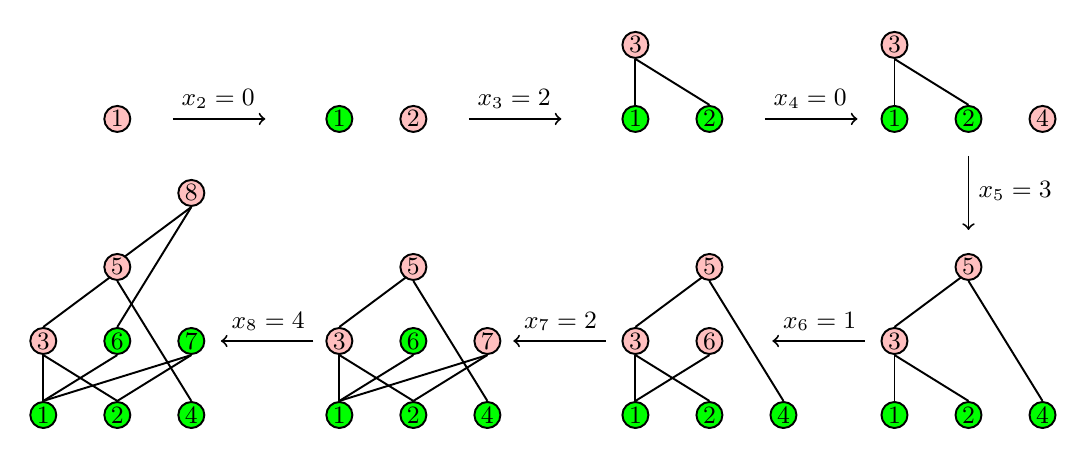
\begin{tikzpicture}[font =\small , scale = 0.47, line width = 0.7pt]
			\tikzmath{\x = -3; \y = -8;\c = 0.38;};
			%1
			\draw[black,fill = pink](1+\x,1)circle(10pt);
			\node at(1+\x,1){1};
			%2 
			\tikzmath{\x = 3;};
			\foreach \i / \j \k in {1/1/1,3/1/2}
			 {	\ifthenelse{\k = 1} 
			 	{\draw[black,fill = green](\i+\x,\j)circle(10pt);}
			 	{\draw[black,fill = pink](\i+\x,\j)circle(10pt);}
					\node at(\i+\x,\j){\k};
			}
		    %3
		    \tikzmath{\x = 11;};
   			\foreach \i / \j \k in {1/1/1,3/1/2}
		    {	
		    	\draw[black,fill = green](\i+\x,\j)circle(10pt);
		    	\node at(\i+\x,\j){\k};
		    }
    		\foreach \i / \j \k in {1/3/3}
		    {	
		    	\draw[black,fill = pink](\i+\x,\j)circle(10pt);
		    	\node at(\i+\x,\j){\k};
		    }
   			\draw(1+\x,1+\c)--(1+\x,3-\c);
	        \draw(3+\x,1+\c)--(1+\x,3-\c);
  			%4
			\tikzmath{\x = 18;};
			\foreach \i / \j \k in {1/1/1,3/1/2}
			{	
				\draw[black,fill = green](\i+\x,\j)circle(10pt);
				\node at(\i+\x,\j){\k};
			}
			\foreach \i / \j \k in {1/3/3,5/1/4}
			{	
				\draw[black,fill = pink](\i+\x,\j)circle(10pt);
				\node at(\i+\x,\j){\k};
			}
   			\draw(1+\x,1+\c)--(1+\x,3-\c);
			\draw(3+\x,1+\c)--(1+\x,3-\c);
			
  			%5
			\tikzmath{\x = 18;};
			\foreach \i / \j \k in {1/1/1,3/1/2,5/1/4}
			{	
				\draw[black,fill = green](\i+\x,\j+\y)circle(10pt);
				\node at(\i+\x,\j+\y){\k};
			}
			\foreach \i / \j \k in {1/3/3,3/5/5}
			{	
				\draw[black,fill = pink](\i+\x,\j+\y)circle(10pt);
				\node at(\i+\x,\j+\y){\k};
			}
			\draw(1+\x,1+\c+\y)--(1+\x,3-\c+\y);
			\draw(3+\x,1+\c+\y)--(1+\x,3-\c+\y);
			\draw (1+\x,3+\c+\y)--(3-0.2+\x,5-\c+0.1+\y);
			\draw (5+\x,1+\c+\y)--(3+\x,5-\c+\y);
			
  			%6
			\tikzmath{\x = 11;};
			\foreach \i / \j \k in {1/1/1,3/1/2,5/1/4}
			{	
				\draw[black,fill = green](\i+\x,\j+\y)circle(10pt);
				\node at(\i+\x,\j+\y){\k};
			}
			\foreach \i / \j \k in {1/3/3,3/5/5,3/3/6}
			{	
				\draw[black,fill = pink](\i+\x,\j+\y)circle(10pt);
				\node at(\i+\x,\j+\y){\k};
			}
			\draw(1+\x,1+\c+\y)--(1+\x,3-\c+\y);
			\draw(3+\x,1+\c+\y)--(1+\x,3-\c+\y);
			\draw (1+\x,3+\c+\y)--(3-0.2+\x,5-\c+0.1+\y);
			\draw (5+\x,1+\c+\y)--(3+\x,5-\c+\y);
			\draw (1+\x,1+\c+\y)--(3+\x,3-\c+\y);
			
  			%7
			\tikzmath{\x = 3;};
			\foreach \i / \j \k in {1/1/1,3/1/2,5/1/4,3/3/6}
			{	
				\draw[black,fill = green](\i+\x,\j+\y)circle(10pt);
				\node at(\i+\x,\j+\y){\k};
			}
			\foreach \i / \j \k in {1/3/3,3/5/5,5/3/7}
			{	
				\draw[black,fill = pink](\i+\x,\j+\y)circle(10pt);
				\node at(\i+\x,\j+\y){\k};
			}
			\draw(1+\x,1+\c+\y)--(1+\x,3-\c+\y);
			\draw(3+\x,1+\c+\y)--(1+\x,3-\c+\y);
			\draw (1+\x,3+\c+\y)--(3-0.2+\x,5-\c+0.1+\y);
			\draw (5+\x,1+\c+\y)--(3+\x,5-\c+\y);
			\draw (1+\x,1+\c+\y)--(3+\x,3-\c+\y);
			\draw (1+\x,1+\c+\y)--(5+\x,3-\c+\y);
			\draw (3+\x,1+\c+\y)--(5+\x,3-\c+\y);
			
  			%8
			\tikzmath{\x = -5;};
			\foreach \i / \j \k in {1/1/1,3/1/2,5/1/4,3/3/6,5/3/7}
			{	
				\draw[black,fill = green](\i+\x,\j+\y)circle(10pt);
				\node at(\i+\x,\j+\y){\k};
			}
			\foreach \i / \j \k in {1/3/3,3/5/5,5/7/8}
			{	
				\draw[black,fill = pink](\i+\x,\j+\y)circle(10pt);
				\node at(\i+\x,\j+\y){\k};
			}
			\draw(1+\x,1+\c+\y)--(1+\x,3-\c+\y);
			\draw(3+\x,1+\c+\y)--(1+\x,3-\c+\y);
			\draw (1+\x,3+\c+\y)--(3-0.2+\x,5-\c+0.1+\y);
			\draw (5+\x,1+\c+\y)--(3+\x,5-\c+\y);
			\draw (1+\x,1+\c+\y)--(3+\x,3-\c+\y);
			\draw (1+\x,1+\c+\y)--(5+\x,3-\c+\y);
			\draw (3+\x,1+\c+\y)--(5+\x,3-\c+\y);
			\draw (3+\x,3+\c+\y)--(5+\x,7-\c+\y);
			\draw (3+0.2+\x,5+\c-0.1+\y)--(5+\x,7-\c+\y);
			
			% labels
			\draw[->] (-0.5,1)--(2,1) node[font = \small,left = 6mm,above]{$x_2 = 0$};
			\tikzmath{\x =8;};
			\draw[->] (-0.5+\x,1)--(2+\x,1) node[font = \small,left = 6mm,above]{$x_3 = 2$};
			\tikzmath{\x =16;};
			\draw[->] (-0.5+\x,1)--(2+\x,1) node[font = \small,left = 6mm,above]{$x_4 = 0$};
			\tikzmath{\x =19;};
			\draw[->] (2+\x,0)--(2+\x,-2) node[font = \small,above = 5mm,right]{$x_5 = 3$};
			\tikzmath{\x =16.2;\y = -6;};
			\draw[->] (2+\x,1+\y)--(-0.5+\x,1+\y) node[font = \small,right = 6mm,above]{$x_6 = 1$};
			\tikzmath{\x =8.2;};
			\draw[->] (3+\x,1+\y)--(0.5+\x,1+\y) node[font = \small,right = 6mm,above]{$x_7 = 2$};
			\tikzmath{\x =0.3;};
			\draw[->] (3+\x,1+\y)--(0.5+\x,1+\y) node[font = \small,right = 6mm,above]{$x_8 = 4$};
		\end{tikzpicture}

\end{document}